%!TEX root = thesis.tex

%:-------------------------- Preamble -----------------------

% Three languages are supported, which will be reflected in the logo on the front page. Pass the appropriate language
% specified as a class option to uit-thesis. Passing any other languages supported by babel will result in the default
% language on the frontpage. If no language is passed, the default is selected.
%  - USenglish (default)
%  - norsk
%  - samin
% The frontpage comes in two variants, Master's thesis and PhD. Master is default, use classoption 'phd' for the PhD version.
\documentclass[USenglish]{uit-thesis}

% Lorem ipsum
\usepackage{lipsum}

\makeglossaries

% Add external glossaryentries
\loadglsentries{acronyms}
\newacronym{api}{API}{application programming interface}\glsunset{api}
\newacronym{2api}{2API}{application programming interface}
\newacronym{d3}{D3}{Data-Driven Documents}
\newacronym{camilla}{CAMILLA}{Camilla is cool!!}
\newacronym{html5}{HTML5}{version 5 of the HyperText Markup Language standard}
\newglossaryentry{thesis}
{
  name=thesis,
  description={is a document submitted in support of candidature for an
    academic degree or professional qualification presenting the author's
    research and findings
    },
}
\newglossaryentry{lage}
{
  name={long ass glossary entry},
  description={is a long ass entry with a lot of text describing the properties of the glossary entry. Hopefully this spans some lines now.
  },
}


\newcommand{\listdefinitionname}{My list of definitions}
\newlistof{definition}{def}{\listdefinitionname}
\newcommand{\definition}[1]{%
  \refstepcounter{definition}%
  \par\noindent\textbf{The Definition~\thedefinition. #1}%
  \addcontentsline{def}{definition}
    {\protect\numberline{\thechapter.\thedefinition}#1}\par%
}

\begin{document}

%:-------------------------- Frontpage ------------------------

\title{From Physical to Virtual Sensors (PVS)}
%\subtitle{Subtitle}			% Optional
\author{Camilla Stormoen}
\thesisfaculty{Faculty of Science and Technology \\ Department of Computer Science}
\thesisprogramme{INF-3983 Capstone Project in Computer Science … December 2017}
%\ThesisFrontpageImage{example_image.jpg}	% Optional

\maketitle

%:-------------------------- Frontmatter -----------------------
\frontmatter

%\begin{dedication}
%To somebody.

%Fuck you very much.
%\end{dedication}

%\begin{epigraph}
%\epigraphitem{Simplicity is prerequisite for reliability.}{Edsger Dijkstra}
%\epigraphitem{Beware of bugs in the above code;\\I have only proved it correct, not tried it.}{Donald Knuth}
%\end{epigraph}

\begin{abstract}
%\lipsum[2-3]
\begin{description}
\item[W3] Whats wrong with the word? / motivation 1-3 setninger
\item[Architecture - 1-3 setninger]
\item [Design- 1-3 setninger]
\item[Implementation - 1-3 setninger]
\item[Experiments - 1-3 setninger]
\item[Results - 1-3 setninger]
\item[Lessons learned/main conclusion - 1-3 setninger]
\item [Kutt heller etterpaa] 
\end{description}

This dissertation present/describe ...
\end{abstract}


%\begin{acknowledgement}
%\lipsum[4-8]
%\end{acknowledgement}

\tableofcontents

%\listofdefinition
\listoffigures

%:-------------------------- Mainmatter -----------------------
\mainmatter

\chapter{Introduction}
\begin{itemize}
\item Mention focus on camera-sensors/data, and not other sensors?!
\item Talk a little bit about COAT in general?
\end{itemize}

This project will develop an abstraction for virtual sensors, and do a prototype of the abstraction on a set of computers with physical sensors.

The purpose is to provide for a more powerful and flexible sensor in the COAT monitoring of the arctic tundra. As such, a fox feeding station is the usage domain to be used for the prototype.


\section{Motivation}
The motivation!
\begin{itemize}
\item W3
\item Problem definition: This project investigated ... x, with the purpose of y.
\end{itemize}

The motivation  behind this project is that no single sensor may cover the sensing needs, and that sensing needs can change rapidly over time. Consequently, there is a need for sensor fusion, and allow for combining sensors at different computers.

\section{Contributions}
What was the contribution?

\section{Assumptions}
AVGRENSE, VIKTIG!!
Something about motivation and stuff

\section{Limitations}
AVGRENSE, VIKTIG!!

\begin{itemize}
\item Mention focus on camera-sensors/data, and not other sensors?!
\end{itemize}

%\begin{itemize}
%\item The first item .
%\end{itemize}

%\begin{enumerate}
%\item The first item
%\end{enumerate}

%\begin{description}
%\item[Entry A] with definition A.
%\end{description}

%\newpage

\iffalse
\subsection{A subsection}

We can use the \ac{api} to \ac{2api} do stuff, and write about what we did in a \gls{thesis}!

This is some stuff, {\sc smallcaps {\em smallcapsemphasized}} {\em regularemphasized}

\Gls{lage}: a test glossary entry.

If the acronym \ac{uit} is displayed, then loadglsentries works.
Hello. This is a test: \ac{camilla}

It is fun to use modern \upsc{OpenMP} technology!\footnote{This is a snarky footnote. Words and etc. Semantic web technologies are technologies that enable semantification of the Web as we know it today. Hopefully this spans some lines now.}

It is fun to use \emph{modern \upsc{OpenMP}} technology! And it is fun to use \ac{d3} and \ac{html5}.

Referencing figure \ref{fig:ex} to test link.\footnote{This is another
footnote.}

\definition{Some other definition}
\fi


\chapter{(Background and) Related Work}
\begin{itemize}
\item Taking Sensor Networks from the Lab to the Jungle
\item Wireless Sensor Networks for Habitat Monitoring
\item Building Virtual Sensors and Actuators over Logical Neighborhoods
\item A virtual sensor system for user-generated, real-time environmental data products
\item Integrating modeling and smart sensors for environmental and human health
\item Capability representation model for heterogeneous remote sensing sensors: Case study on soil moisture monitoring
\item Dice: Monitoring Global Invariants with Wireless Sensor Networks 
\\ \em{Ştefan Gună, Luca Mottola, and Gian Pietro Picco. 2014. DICE: Monitoring global invariants with wireless
sensor networks. ACM Trans. Sensor Netw. 10, 4, Article 54 (April 2014), 34 pages.}
DOI: http://dx.doi.org/10.1145/2509434
\end{itemize}


\section{Virtual Sensors}
A virtual sensor is a constructed sensor unlike/dissimliar/contrary to a physical sensor as described by S. Kabadayi et. al.\cite{VirtualSensors2006}. They are used in place of the real sensors where they read real physical sensor data and calculate the outputs by using some processing models.

In this project the biologists want to search for pictures of a specific animal from different locations in the Arctic Tundra. A virtual sensor would collect data from the physical sensors and then return those images that are equivalent to the biologists input.

Ciciriello et. al.\cite{Ciciriello} describes virtual nodes which are programming abstractions that should simplify the development of decentralized wireless sensor network applications. Their system enable access to the data by a given set of sensors and making it into one virtual sensor that a programmer can interact with.
The physical nodes are abstracted and specified using logical neighborhoods \cite{Mottola2006}\cite{Mottola2006_2}. The nodes are combined in a logical neighborhood that are specified based on their characteristics by the programmer. 

TinyOS \cite{TinyOS}

Our work relies on physical sensor data which is already in a data storage, and not directly from the physical sensors.


\section{Something}



\chapter{Architecture}
This chapter describes the architecture of the system.
There are 6 components in the system: physical sensors, data storage, fused data, virtual sensors and the user. However, the main components in the system are the data storage, the fused data, the virtual sensors and the user.
The architecture of the system is presented in Figure \ref{fig:architecture}.

\begin{figure}
\centering
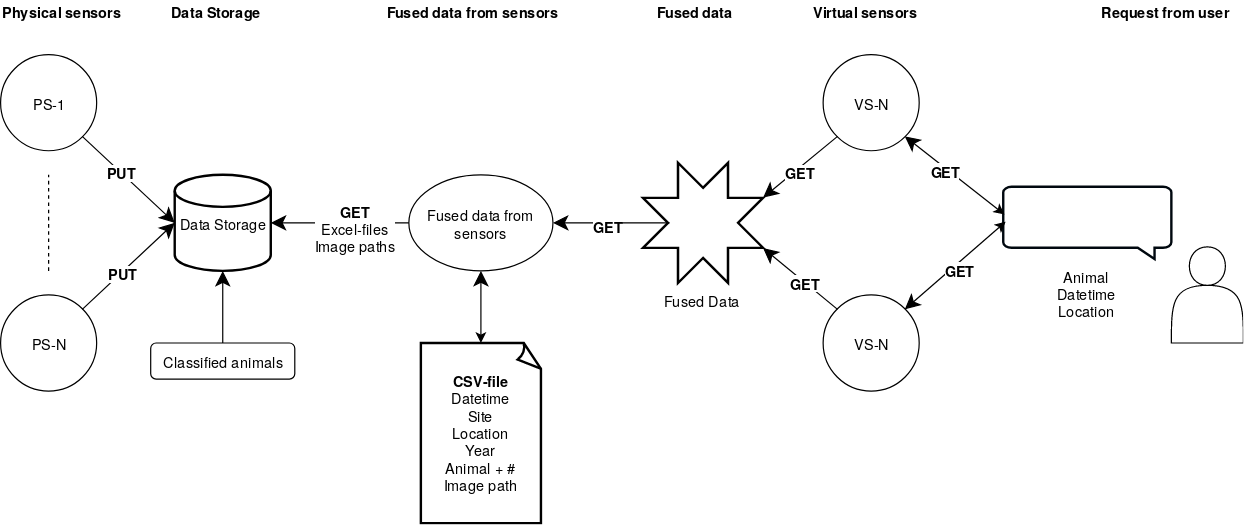
\includegraphics[width=\textwidth]{Architecture2.png}
\caption{Figure showing the system architecture.}
\label{fig:architecture}
\end{figure}


\section{Physical Sensors and Data Storage}
The physical sensors transmit their data to the data storage, so the data storage consists of several set of images from the different bait-camera sensors. These pictures are organized by the year they where taken and also where the camera was placed in the Arctic Tundra in Finnmark, Norway. 
The data store also contains several excel-sheets containing information about each picture structured by the location of the physical bait-camera sensor position.

\section{Fused Data}
The fused data retrieves it's data from the data storage and store the fused data into a Comma-Separated Value (CSV) file on demand. The fused data is the image-path from all the directories in the data storage combined with necessary information from the excel-sheet such as date-time, location, site, year, what kind of animal was in the image and also how many animals there was.

\section{Virtual Sensors}
The virtual sensors are divided multiple sensors representing different animals that scientists are interested in, e.g. one raven-sensor, one red fox-sensor and one golden eagle-sensor.
The user types in what animal it wants to see, where it is and the date-time and the search is redirected to the sensor related to that specific animal. The virtual sensor receive its result from the fused data from the CSV-file.

\section{Result from Virtual Sensor to User}
A user wants to retrieve images from the data store.
The user interacts with a user application. This application takes care of the communication to the virtual sensors. When a user gives a command, the user application sends it to one of the virtual sensors, the virtual sensor retrieve data from the fused data as described in the section above, and deliver the response back to the user. The image(s) are displayed through an image-vision.


\chapter{Design}
Client/Server, p2p, put/get, pub/sub, protokoller etc..
BESKRIV INTERAKSJONEN MELLOM ENHETENE!!

Virtual sensors probably uavhengige prosesser, ikke threads ettersom man evt vil addere flere sensorer og unnga a starte alle sensorer på nytt igjen..
Er de virtuelle sensorene servere eller client/publisher?

In this chapter we will look at the design of the environment. We will present the design of the data storage, the fused data the virtual sensors and the user application. Figure \ref{fig:design} shows the design of the system. The arrows indicates the communication lines. The dotted arrows show how the data storage is structured with files and pictures.


\begin{figure}
\centering
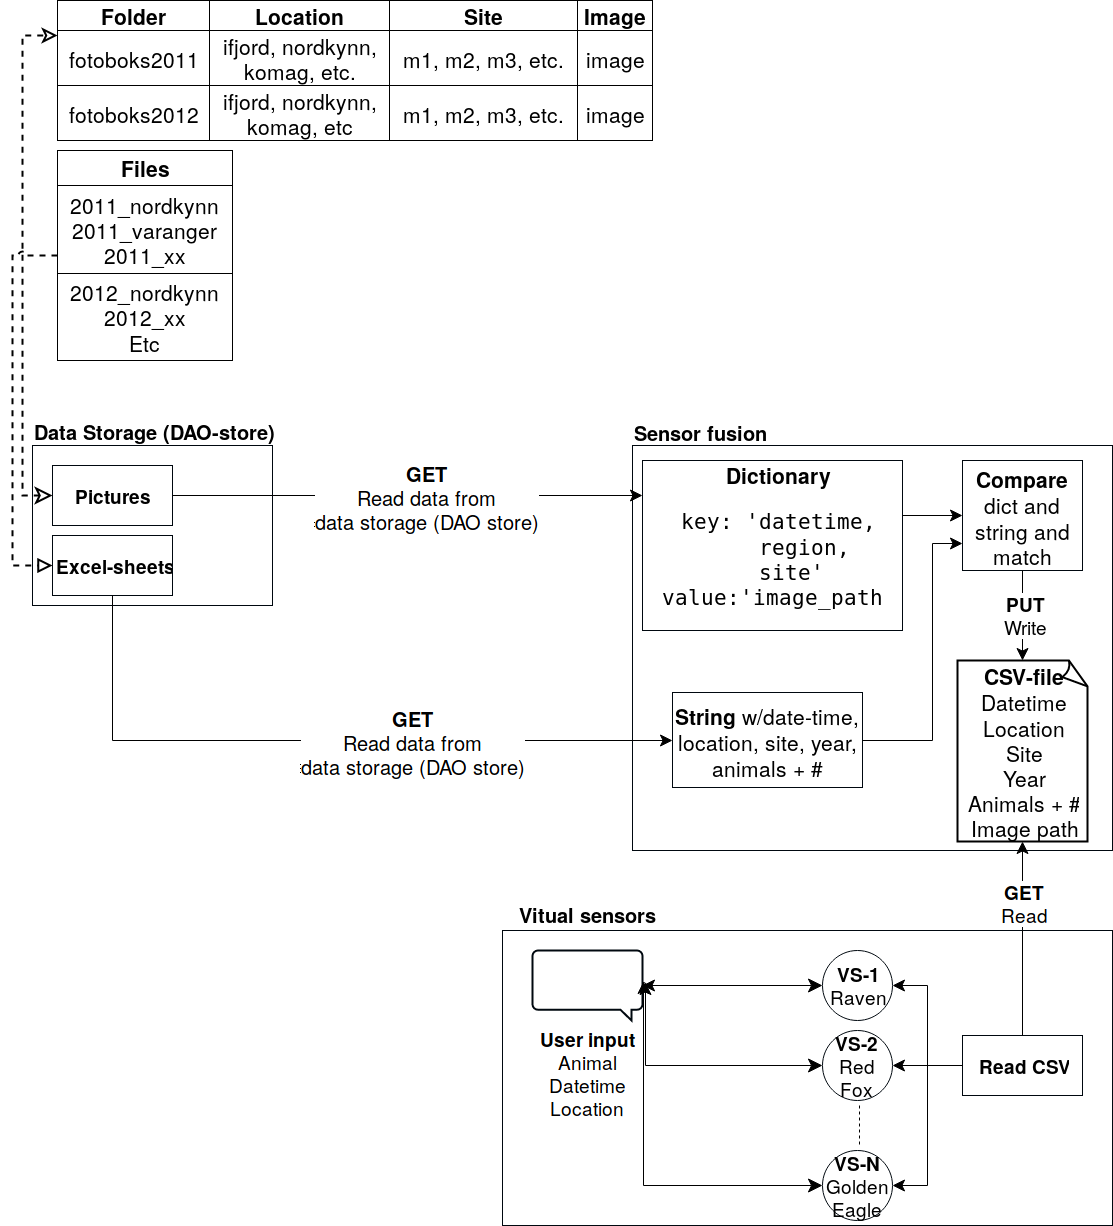
\includegraphics[width=\textwidth]{Design.png}
\caption{Figure showing the system design.}
\label{fig:design}
\end{figure}

\section{Data Storage and Fused Data from Sensors}
The dataset from the physical sensors contains over 1.6 millions of pictures from 2011 to 2016 taken from the Arctic Tundra in Finnmark, Norway. The physical sensors are placed at different areas in the Arctic Tundra such as Nordkynn, Komag, Nyborg, Stjernevann and Gaissene.
The excel-sheets contains from 17 000 to 70 000 rows with information about each picture taken.

The excel-sheet in the data storage contains a pictures location, date-time, site and year, but it did not contain any filename or a filepath. We then had to find a method to find out which images correspond to which field/row in the excel-sheet. Fortunately, each image had metadata stored in Exchangeable Image File Format (EXIF). We recursively traversing the directories where pictures are located and read date and time for each picture which is stored in a Python dictionary, like a key-value store, with date and time as key and image-path as value.


Date and time from each image is extracted and stored in a dictionary together with the necessary information from the excel-sheet.


\section{Fused Data from Sensors}




Rekursiv traversering av directories og leser metadata fra bildene (ca 1,6 mill bilder)) - Lagres i en dictionary hvor datetime og sted er key og image pathen er value).


FRA HÅVARDS MASTER: The csv files did not contain any filenames,
only image metadata and animal classifications, so we had to get creative
to find out which images the annotations corresponded to. Fortunately, each
image had metadata stored in Exchangeable Image File Format ( exif ). We
created a Python script to extract the date and time from each image, along
with camera information, to match them with the annotations. This was quite
a time-consuming task because of the number of images to process.

Disse sammenlignes og de som matcher blir skrevet til en CSV-fil.
\section{Virtual Sensors}
\section{User}
The user-application is the connection between  the user and the virtual sensors. It gets input from the user and sends a request to the virtual sensor based on its input. The user-applications goal is to make an interface that is easy to use and to show images that the user want to see.
The user only need to specify the following 3 paramteres for the virtual sensor:
\begin{description}
\item [Animal]
\item [Date-time]
\item [Location]
\end{description}

\begin{itemize}
\item Animal:
\item Date-time:
\item Location:
\end{itemize}



\iffalse 
\begin{table}
\centering
\begin{tabular}{|l|l|}
\hline
Content left & Content right\\
\hline
\end{tabular}
\caption{A table}
\end{table}


%\newpage

\begin{lstlisting}[frame=single,caption={Small C program},language=C]
#include "stdio.h"
#define e 3
#define g (e/e)
#define h ((g+e)/2)
#define f (e-g-h)
#define j (e*e-g)
#define k (j-h)
#define l(x) tab2[x]/h
#define m(n,a) ((n&(a))==(a))

long tab1[]={ 989L,5L,26L,0L,88319L,123L,0L,9367L };
int tab2[]={ 4,6,10,14,22,26,34,38,46,58,62,74,82,86 };

main(m1,s) char *s; {
  int a,b,c,d,o[k],n=(int)s;
  if(m1==1){ char b[2*j+f-g]; main(l(h+e)+h+e,b);
    printf(b); }
  else switch(m1-=h){
    case f:
      a=(b=(c=(d=g)<<g)<<g)<<g;
      return(m(n,a|c)|m(n,b)|m(n,a|d)|m(n,c|d));
    case h:
      for(a=f;a<j;++a)
        if(tab1[a]&&!(tab1[a]%((long)l(n))))
          return(a);
    case g:
      if(n<h)return(g);
      if(n<j){n-=g;c='D';o[f]=h;o[g]=f;}
      else{c='\r'-'\b';n-=j-g;o[f]=o[g]=g;}
      if((b=n)>=e)
        for(b=g<<g;b<n;++b)o[b]=o[b-h]+o[b-g]+c;
      return(o[b-g]%n+k-h);
    default:
      if(m1-=e) main(m1-g+e+h,s+g); else *(s+g)=f;
      for(*s=a=f;a<e;) *s=(*s<<e)|main(h+a++,
      (char *)m1);

    }
}
\end{lstlisting}

\fi

\chapter{Implementation}
%\lipsum[3-4]
Threads, data structures, language ...
Pandas (dataframe \footnote{\url{https://pandas.pydata.org/pandas-docs/stable/generated/pandas.DataFrame.html}} \footnote{\url{http://pandas.pydata.org/pandas-docs/stable/}}), CV2 (show image), exifread, Python 2.7, missing testing (CPU, memory, time?)


The system is implemented and written in Python 2.7\footnote{\url{https://www.python.org/}} because .. (frameworks available in this language??).

To visualize/show pictures, a Python library called OpenCV \footnote{\url{https://opencv-python-tutroals.readthedocs.io/en/latest/}} was implemented.
To read exif/metadata from pictures, we used a Python library called exifread 2.1.2 \footnote{\url{https://pypi.python.org/pypi/ExifRead}}.

\chapter{Evaluation} 
metrics, define (CPU, memoury, lantecy.), benchmarks (mirko, kernel...
How to measure, where done, PSEUDOCODE

\begin{itemize}
\item Time: Finding folders and metadata takes:  1:43:13.488799,
Reading excel file takes:  0:00:17.413845,
Comparing takes:  4:43:30.705587,
Overall time is  6:27:01.608355.
Med alle bilder m/metadata og hele fotoboks2011\_nordkynn\_nordkynn.2011.xlsx.

\item New time: Finding folders and metadata takes:  1:46:17.406581
Reading excel file takes:  0:01:07.686779
Comparing takes:  19:03:11.177869
Overall time is  20:50:36.271415
Med alle bilder m/mETADATA og hele nordkynn og varanger

\item "Concurrent" python find\_folder\_ok\_concurrent.py 
Finding folders and metadata takes:  1:30:50.250732
Reading excel file takes:  0:00:18.127597
Comparing takes:  4:18:33.368199
Overall time is  5:49:41.746759
\\ -- Pool(processes=4)
FRA fotoboks2011\_nordkynn\_nordkynn.2011.xlsx

\item "Concurrent" igjen
Finding folders and metadata takes:  1:44:18.788013
Reading excel file takes:  0:00:17.269817
Comparing takes:  3:54:23.483186
Overall time is  5:38:59.541248
-- Pool(processes=100)
\\ FRA fotoboks2011\_nordkynn\_nordkynn.2011.xlsx

This chapter describes the experimental setup and metrics used to evaluate the implemented system. 

\end{itemize}
\section{Experimental Setup}
All experiements was done on a Lenovo ThinkCenter with an Intel® Core™ i5-6400T CPU @ 2.20GHz × 4, Intel® HD Graphics 530 (Skylake GT2), 15,6 GiB memory and 503 GB disk. It ran on Ubuntu 17.04 64-bit.

\section{Something!?}
\section{Results}
What does the result say?
Each experiment, result, meaning

\chapter{Discussion}
Idea, architecture, design, results, other solutions, "arch have scale-problem?".

\section{Architecture}
\subsection{Other solutions}
\begin{itemize}
\item Virtual sensors probably uavhengige prosesser, ikke threads ettersom man evt vil addere flere sensorer og unnga a starte alle sensorer på nytt igjen..
\item Updates of "database" in background, not on demand -> future work
\end{itemize}

\section{Design}
\subsection{Other solutions}
\begin{itemize}
\item hash-map instead of multiple lists with different animals. hash on animal and/or place
\item parallel/concurrent program when doing metadata-collecting and reading from excel-sheet and writing to csv
\item FRA HÅVARDS MASTER: The csv files did not contain any filenames,
only image metadata and animal classifications, so we had to get creative
to find out which images the annotations corresponded to. Fortunately, each
image had metadata stored in Exchangeable Image File Format ( exif ). We
created a Python script to extract the date and time from each image, along
with camera information, to match them with the annotations. This was quite
a time-consuming task because of the number of images to process.
\end{itemize}



\chapter{Contributions}
Combine with conclusion??
\chapter{Conclusion}
\section{Contributions?}
\section{Future Work}

\chapter{Future Work?}

\chapter{Appendix?}
readme, source code, dataset measurement RAW
\backmatter


%%% BIBLOGRAPHY

\newpage{}

\begin{thebibliography}{9}

\bibitem{VirtualSensors2006}
S. Kabadayi and A. Pridgen and C. Julien
\newblock {\em Virtual Sensors: Abstracting Data from Physical Sensors}, 2006,
\newblock in {\em 2006 International Symposium on a World of Wireless, Mobile and Multimedia Networks(WoWMoM'06), 6 pp.-592}.


\bibitem{Ciciriello}
Ciciriello, Pietro and Mottola, Luca and Picco, Gian Pietro
\newblock {\em Building Virtual Sensors and Actuators over Logical Neighborhoods}, 2006,
\newblock in {ACM, 19--24}.
\newblock {\em \url{http://doi.acm.org/10.1145/1176866.1176870}}.


\bibitem{TinyOS}
Hill, Jason and Szewczyk, Robert and Woo, Alec and Hollar, Seth and Culler, David and Pister, Kristofer
\newblock {\em System Architecture Directions for Networked Sensors}, 2000,
\newblock in {\em  ASPLOS-IX: Proc. of the 9 nt Int. Conf. on
Architectural Support for Programming Languages and
Operating Systems}, pages 93–104, 2000.


\bibitem{Mottola2006}
Mottola, Luca and Picco, Gian Pietro
\newblock {\em Logical Neighborhoods: A Programming Abstraction for Wireless Sensor Networks}, 2006,
\newblock in {\em  Distributed Computing in Sensor Systems: Second IEEE International Conference, DCOSS 2006, San Francisco, CA, USA, June 18-20, 2006. Proceedings}, pages 150--168, 2000.
\newblock {\em \url{http://.............}}.


\bibitem{Mottola2006_2}
Mottola, Luca and Picco, Gian Pietro
\newblock {\em Programming Wireless Sensor Networks with Logical Neighborhoods}, 2006,
\newblock in {\em  Proceedings of the First International Conference on Integrated Internet Ad Hoc and Sensor Networks},
 series = {InterSense '06}, pages 150--168, 2000.
\newblock {\em \url{http://doi.acm.org/10.1145/1142680.1142691}}.




\end{thebibliography}

\end{document}

